\documentclass{article}

\usepackage{geometry}
\geometry{a4paper,margin=1in,}

\usepackage{hyperref}
\usepackage{graphicx}
\usepackage{float}

\title{COSC345 App Proposal}
\author{Name 1 (ID 1) Name 2 (ID 2) \\ Name 3 (ID 3) Louis Whitburn (2548261)}
\date{\today}

\begin{document}
	\maketitle
	
	We are building an android app to display university course material. This will be targeted towards displaying content from cs.otago.ac.nz primarily. It will provide an easy to view format of each paper for mobile devices. Information will be pulled from the websites themselves and formatted.
	
	Our team consists of: (previous years people wrote quite a bit about each member)
	(we should probably work out roles and talk about our strengths or something)
	Louis Whitburn – 
	Garth Wales – I am happy to work on design aspects
	BJ - 
	Damian Soo – 

	We are using Kotlin and intend to target Android API level 28 (Android version 9). The app will function by using common formats of each department to guess the locations of papers lecture slides or other information. An example being cs.otago.ac.nz/(papercode)/lectures.php is where most COSC papers have their lecture slide pdfs. The app will then cache and display the information from these pages.

	We will begin by implementing PDF viewing capabilities and pulling the PDF from one specific paper, then expand into a better dynamic system. 

	It will take roughly 5 months of part time work to complete the app, including some time for unexpected issues or setbacks.
	
	\begin{figure}[h!]
		\centering
		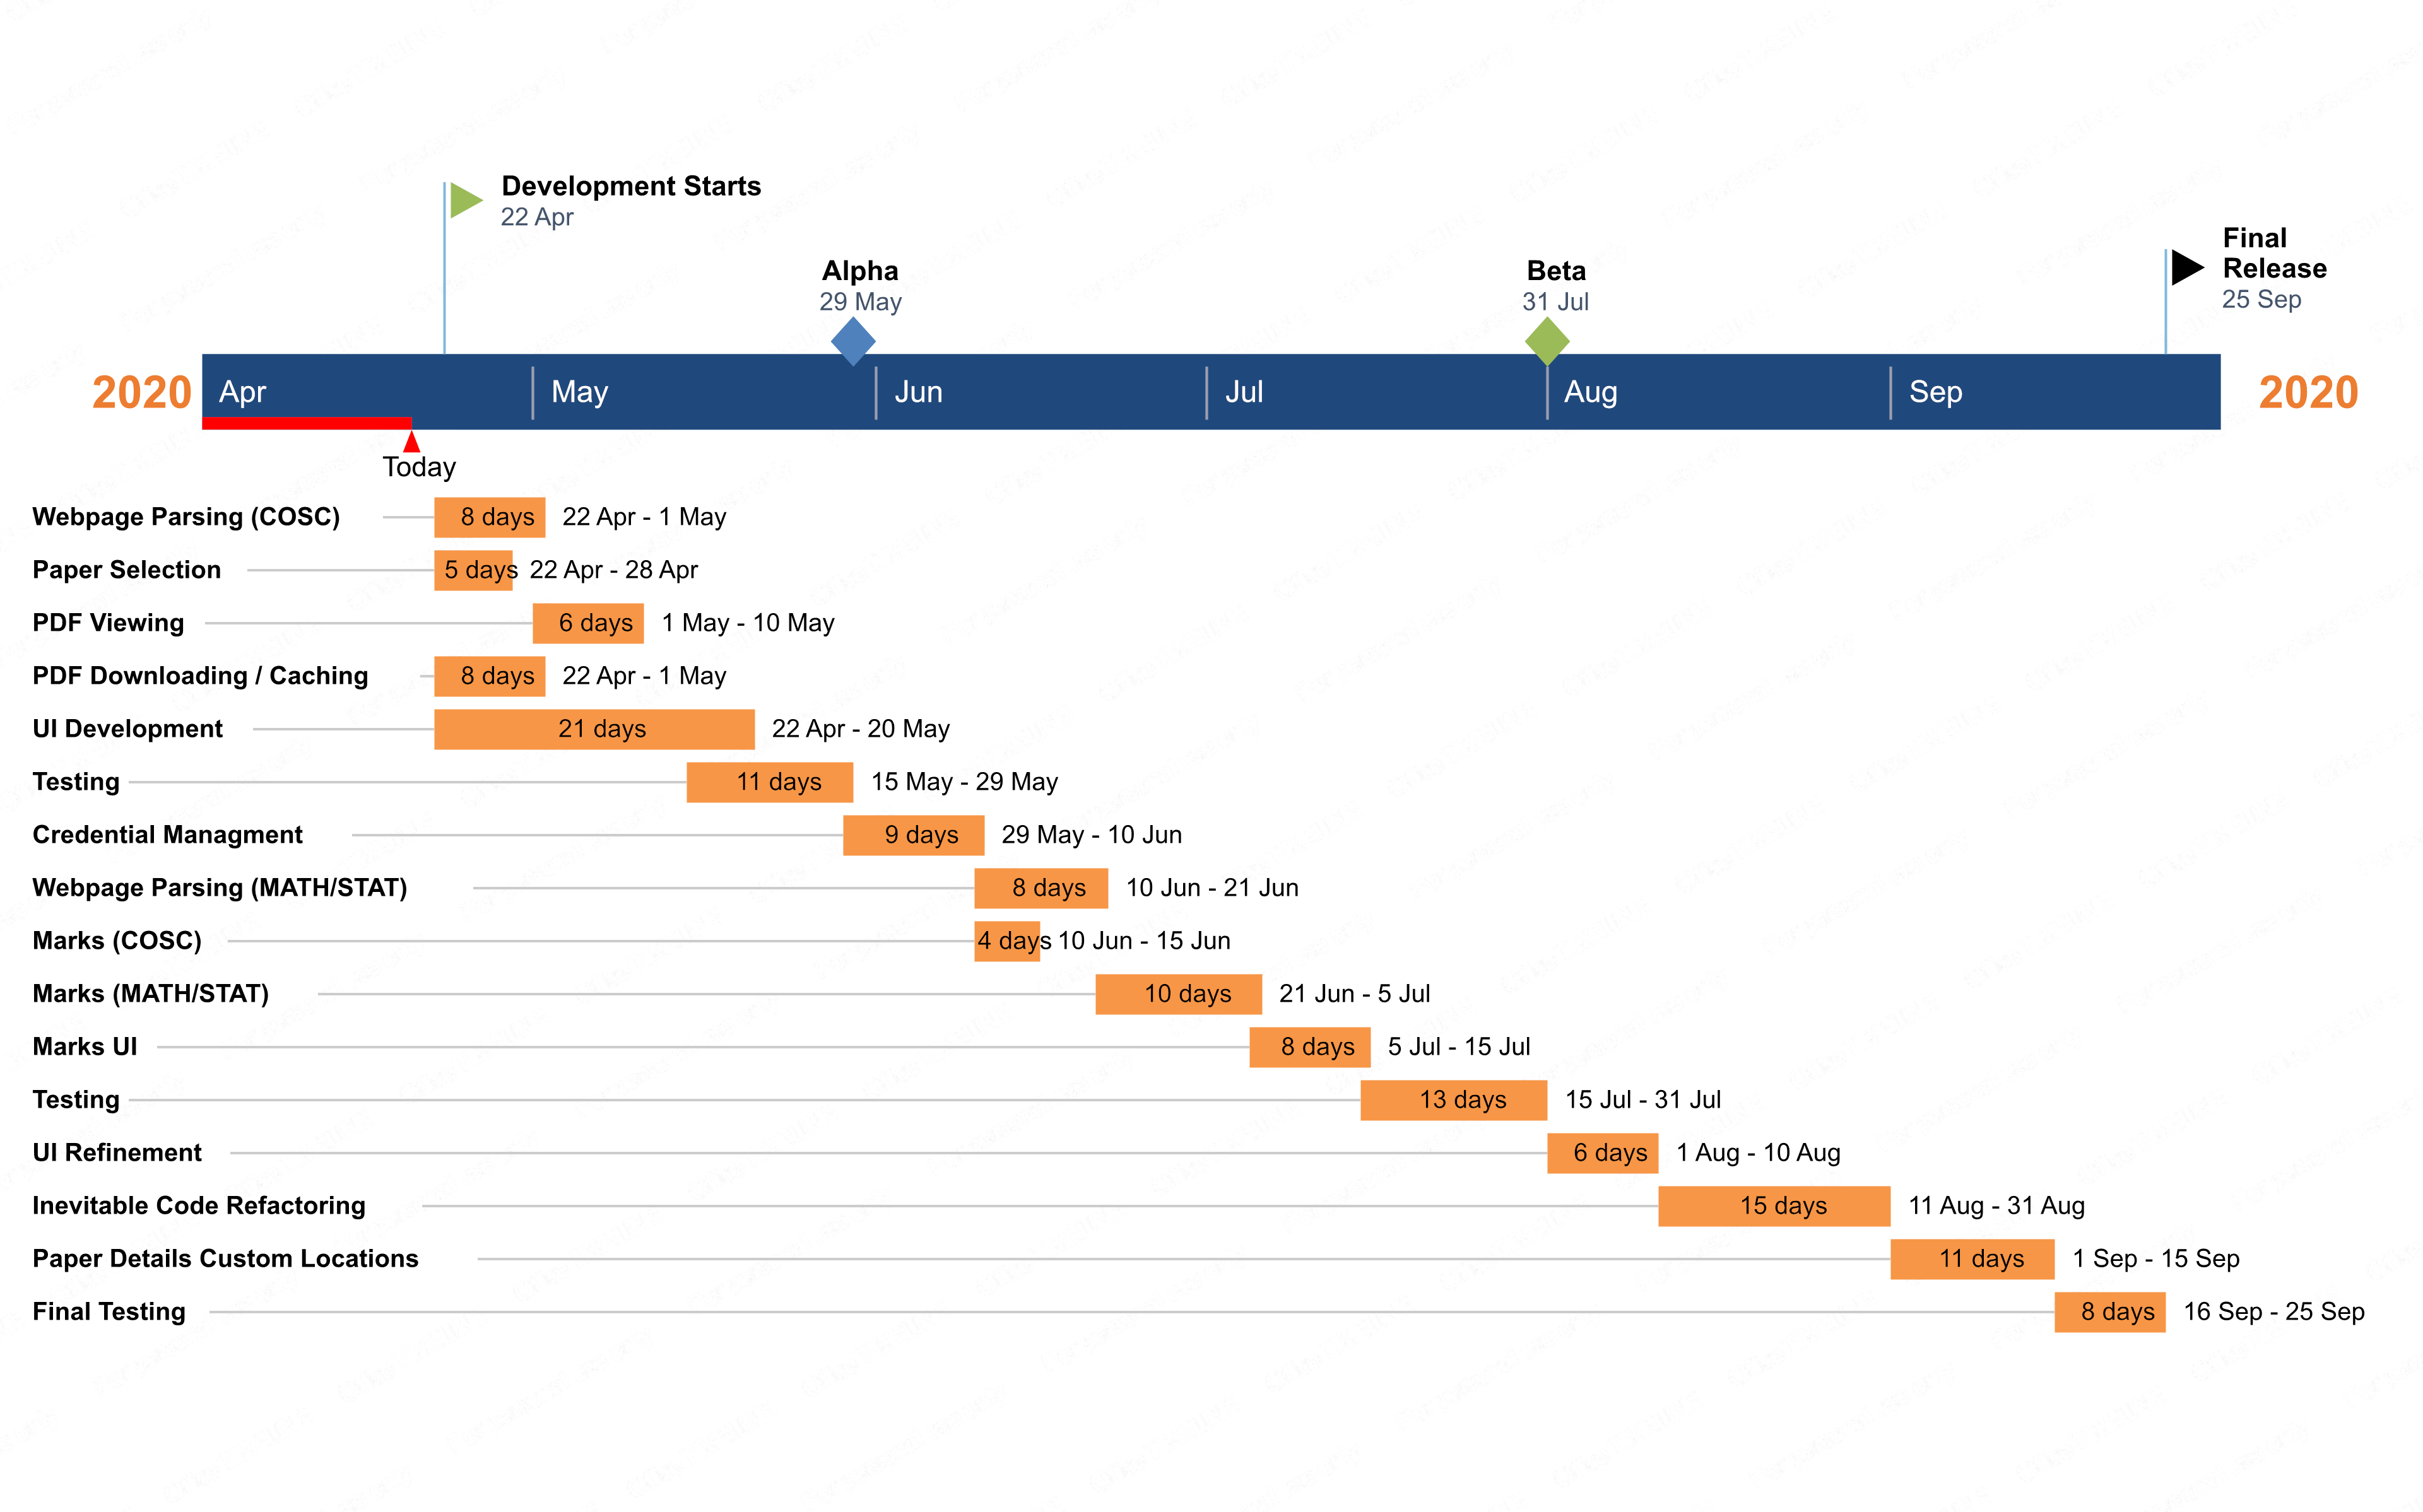
\includegraphics[width=\linewidth]{chart.png}
	\end{figure}
	
	Our biggest risk is website formats changing causing the app to no longer function. Either with individual papers changing the layout or using different systems such as blackboard. For blackboard we will explore credential storage to access pages behind passwords to ensure we have full coverage.
	
	The establishment already has websites such as cs.otago.ac.nz. However, these websites are rubbish on mobile devices and they do not provide any mobile solutions. We will irritate the establishment by creating a better alternative to their existing solutions. We will be doing this with our source code hosted on the establishments own gitlab server to add insult to injury.
\end{document}